\documentclass[a4paper,12pt]{article}

\usepackage[utf8x]{inputenc}
\usepackage[T2A]{fontenc}
\usepackage[english, russian]{babel}

% Опционно, требует  apt-get install scalable-cyrfonts.*
% и удаления одной строчки в cyrtimes.sty
% Сточку не удалять!
\usepackage{cyrtimes}

% Картнки и tikz
\usepackage{graphicx}
\usepackage{tikz}
\usetikzlibrary{snakes,arrows,shapes}


% Некоторая русификация.
\usepackage{misccorr}
\usepackage{indentfirst}
\renewcommand{\labelitemi}{\normalfont\bfseries{--}}

% Увы, поля придётся уменьшить из-за листингов.
\topmargin -1cm
\oddsidemargin -0.5cm
\evensidemargin -0.5cm
\textwidth 17cm
\textheight 24cm

\sloppy

% Оглавление в PDF
\usepackage[
bookmarks=true,
colorlinks=true, linkcolor=black, anchorcolor=black, citecolor=black, menucolor=black,filecolor=black, urlcolor=black,
unicode=true
]{hyperref}

\usepackage{listings}

% Значения по умолчанию
\lstset{
  basicstyle=\ttfamily,
  columns=fullflexible,
  breaklines=true,       % переносить длинные строки
%  inputencoding=koi8-r,
  showspaces=false,      % показывать пробелы подчеркиваниями -- идиотизм 70-х годов
  showstringspaces=false,
  showtabs=false,        % и табы тоже
  stepnumber=1,
  tabsize=4,              % кому нужны табы по 8 символов?
  frame=single
}

% Свой язык для задания грамматик в BNF
\lstdefinelanguage[]{Pixel}[]{}{
  morekeywords={TRANSACTION_ID,ADVERTISER_ID,OFFER_CODE,OFFER_CODE1,OFFER_CODE2,OFFER_CODE3,COST},
}[keywords,comments,strings]

% Для исходного кода в тексте
\newcommand{\Code}[1]{\texttt{#1}}

\newcommand{\heymoose}{<<HeyMoose!>>}

\title{Руководство \\ по интеграции с системой \heymoose \\ с использованием XML-сервиса}
% \date{(версия от 4 сентября 2012)}

\begin{document}

\maketitle

\thispagestyle{empty}

\newpage

\tableofcontents

\newpage

\section{Используемые термины и понятия}

\textbf{Рекламная кампания}~--- рекламное предложение, которое размещает рекламодатель в системе \heymoose. Партнеры сети \heymoose{} получают доступ к материалам и описанию рекламной кампании и размещают их на своих площадках.

\textbf{Рекламная площадка}~--- веб-сайт или рекламная сеть, где партнер размещает материалы рекламной кампании.

\textbf{Посадочная страница (Landing Page)}~--- страница на сайте рекламодателя, на которую переходит пользователь с рекламной площадки.

\textbf{Эксклюзивный товар}~--- товар в интернет-магазине при покупке которого пользователем, перешедшим на сайт магазина от системы \heymoose{}, партнёр, приведший этого пользователя, получает повышенное вознаграждение. 

\newpage

\section{Преимущества XML-интеграции}

Интеграция с системой \heymoose{} с использованием XML-сервиса требуется преимущественно для интернет-магазинов, которые желают платить партнёрам вознаграждение, подсчитываемое как процент от покупки пользователями каждого товара.

Одним из основных достоинств XML-интеграции с \heymoose{} является возможность указания т.н. \textit{эксклюзивных товаров}, вознаграждение за которые выше, чем в других партнёрских сетях. Выгода для рекламодателя заключается в том, что партнёры стремятся рекламировать именно эксклюзивные товары, тем самым повышая средний чек интернет-магазина или увеличивая продажи товаров определенного типа.

Интеграция с использованием XML-сервиса (\textit{server-to-server}) является более сложной схемой, в отличие от интеграции с использованием подтверждающего пикселя, поскольку требует написания серверного кода. Однако, данная схема обладает рядом неоспоримых преимуществ:

\begin{itemize}
\item \textit{идентификатор перехода (токен)} хранится на стороне рекламодателя (в базе данных, в скрытых переменных или в параметрах URL), что дает большую надежность по сравнению с хранением токена в Cookies пользователя;
\item при выходе из строя сервера одной из сторон (интернет-магазина или партнёрской сети) статистика продаж сохраняется, и не происходит потерь отслеживаемых заказов;
\item основной единицей оплаты является не заказ, а товар, что дает большую гибкость в подсчете партнёрского вознаграждения и возможность подтверждать и отменять не весь заказ, а каждый товар в заказе по отдельности;
\item сверка заказов (подтверждение или отмена товаров в заказе) происходит в автоматическом режиме и не требует участия человека с обеих сторон;
\item собранная по товарам статистика позволяет получить информацию о том, какие товары в магазине продаются лучше или хуже;
\item партнёры заинтересованы в продаже эксклюзивных товаров и, тем самым, в повышении среднего чека магазина;
\item партнёры обладают подробной информацией о каждом товаре и могут делать более точную их рекламу, соответствующую тематике рекламных площадок.
\end{itemize}

\section{Схема взаимодействия с системой \heymoose}

Интеграция с системой \heymoose{} с использованием XML-сервиса подразумевает несколько подготовительных этапов:
\begin{enumerate}
\item Рекламодатель регистрируется в системе \heymoose{}.
\item Рекламодатель высылает список \textit{всех} товаров в интернет-магазине в специальном формате YML (Yandex Market Language), указывая при этом, какие товары являются эксклюзивными, и ставку за каждый товар. На основе этого списка в системе \heymoose{} создается рекламная кампания интернет-магазина.
\item Рекламодатель на своей стороне реализует XML-сервис, возвращающий все заказы, сделанные пользователями, перешедшими от рекламных площадок системы \heymoose{}, за последние 30 дней.
\end{enumerate}

Общая схема взаимодействия интернет-магазина рекламодателя с системой \heymoose{} выглядит следующим образом:

\begin{enumerate}
\item Партнер размещает на \textit{рекламной площадке} описание рекламной кампании и специальную ссылку системы \heymoose. Посетитель рекламной площадки видит это описание и переходит по партнёрской ссылке.
\item Сервер \heymoose{} перенаправляет (redirect) пользователя на \textit{посадочную страницу} рекламной кампании, передавая при этом специальные GET-параметры:
	\begin{itemize}
	\item \textbf{\_hm\_token}~--- идентификатор (token) перехода в системе \heymoose{};
	\item \textbf{\_hm\_ttl}~--- время жизни Cookie в днях (необязательный параметр для данной схемы).
	\end{itemize}
\item Сервер интернет-магазина сохраняет переданный токен каким-либо образом.
\item Пользователь совершает заказ одного или нескольких товаров в интернет-магазине. Интернет-магазин сохраняет соответствие заказа с токеном, переданным на шаге (2).
\item Сервер \heymoose{} с некоторой периодичностью опрашивает реализованный XML-сервис рекламодателя, отслеживая вновь созданные заказы.
\item Если один или несколько товаров в заказе отменяются, их статус меняется на <<отменён>> в возвращаемом XML. Если заказ отменяется, статус всех товаров в заказе изменяется на <<отменён>>. Если заказ подтверждается, статус всех (неотменённых) товаров в заказе меняется на <<подтверждён>>. Система \heymoose{} видит изменение статуса и также производит отмену или подтверждение товаров в своей статистике.
\end{enumerate}

\section{Этапы интеграции}

В этом разделе подробно описаны основные действия, которые должен совершить рекламодатель для успешной интеграции с системой \heymoose{} с использованием XML-сервиса.

\subsection{Регистрация в системе \heymoose{}}

Прежде всего необходимо зарегистрироваться в системе \heymoose{} в качестве рекламодателя. Для этого нужно перейти по ссылке \href{http://heymoose.com/register/advertiser/}{http://heymoose.com/register/advertiser/}, заполнить все поля в форме и нажать на кнопку <<Зарегистрироваться>>. После успешной регистрации необходимо подтвердить введенный адрес электронной почты, перейдя по ссылке в полученном письме.

После проделанных действий необходимо сообщить ваш логин (адрес электронной почты, с которым вы зарегистрировались) менеджеру \heymoose{}, который с вами работает.

\subsection{Список товаров в формате YML}

Список товаров необходимо возвращать в специальном формате YML, используемом для системы <<Яндекс.Маркет>>. Спецификацию формата и описание всех полей можно найти по адресу \href{http://partner.market.yandex.ru/legal/tt/}{http://partner.market.yandex.ru/legal/tt/}.

Для системы \heymoose{} в описание каждого товара необходимо добавить два параметра:
\begin{itemize}
\item \textbf{hm\_exclusive}~--- если true, товар считается эксклюзивным, иначе (если false или параметр не задан) товар считается обычным.
\item \textbf{hm\_value}~--- размер выплаты в пользу системы \heymoose{} за данный товар. Параметр имеет атрибут \textbf{unit}, который может принимать следующие значения:
	\begin{itemize}
	\item \textit{percent}~--- значение параметра \textbf{hm\_value} является процентной ставкой (оплата в пользу \heymoose{} подсчитывается как процент от стоимости товара);
	\item \textit{fixed}~--- значение параметра \textbf{hm\_value} является фиксированной ставкой (в рублях и копейках, разделенных точкой).
	\end{itemize}
\end{itemize}

Пример измененного описания товара в формате YML приведен ниже. В данном примере последние два параметра означают, что товар является эксклюзивным и при его покупке в пользу системы \heymoose{} будет выплачена сумма в размере 15\% от стоимости товара.

\begin{footnotesize}
\begin{verbatim}
  <offer id="1234" available="true">
      <url>http://shop.example.com/product/1234/</url>
      <price>800</price>
      <currencyId>RUR</currencyId>
      <categoryId>9995</categoryId>
      <picture>http://shop.example.com/pics/1234.jpg</picture>
      <delivery>true</delivery>
      <name>Сумка женская</name>
      <vendorCode>400</vendorCode>
      <description>Кожаная сумка 40х60 см</description>
      <param name="hm_exclusive">true</param>
      <param name="hm_value" unit="percent">15</param>
  </offer>
\end{verbatim}
\end{footnotesize}

Требования к списку товаров интернет-магазина в формате YML следующие:
\begin{enumerate}
\item В данном списке должны содержаться \textbf{все} товары интернет-магазина (не только эксклюзивные) с указанными в параметрах ставками.
\item Список должен храниться по определенному адресу на сервере рекламодателя и быть всегда доступным и актуальным (может предоставляться также в виде сервиса). Система \heymoose{} будет производить опрос списка с некоторой периодичностью.
\item Время ответа от сервера рекламодателя при запросе списка не должно превышать 5~секунд.
\item Если доступ к списку товаров закрыт извне, необходимо открыть его для IP-адресов серверов \heymoose{}.
\end{enumerate}

Если для вашего интернет-магазина невозможно выполнить какие-либо требования или добавить параметры в документ YML, пожалуйста, свяжитесь с нашими менеджерами.

Через некоторое время после того, как вы сформировали список товаров согласно требованиям и сообщили адрес его расположения нашим менеджерам, в вашем личном кабинете создастся рекламная кампания вашего интернет-магазина (рис.~\ref{fig:offer}).

\begin{figure}[!ht]
\centering
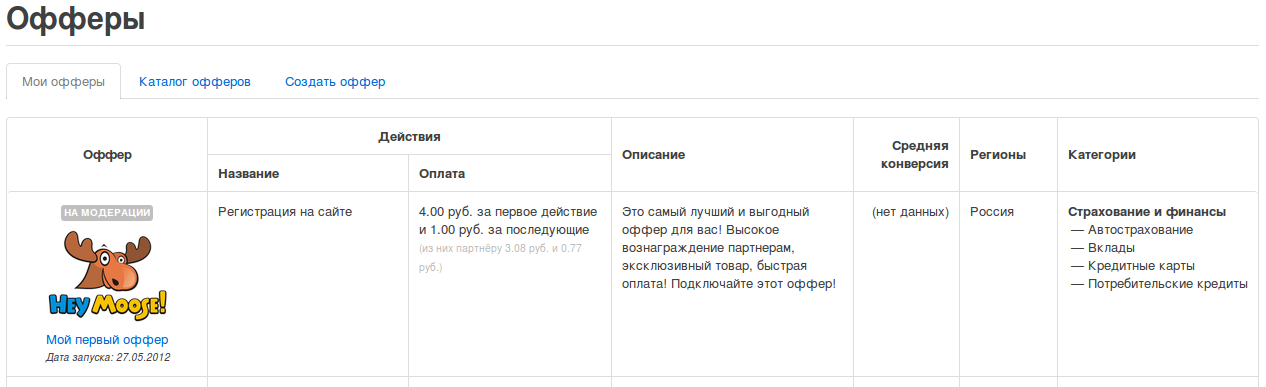
\includegraphics[width=\textwidth]{include/offer.png}
\caption{Созданная кампания в списке офферов.}
\label{fig:offer}
\end{figure}

При нажатии на логотип оффера, вы попадете на страницу описания рекламной кампании, где можете настраивать и управлять созданной рекламной кампанией.

\subsection{Отслеживание пользователей}

При переходе пользователя на сайт интернет-магазина от системы \heymoose{} на посадочную страницу передается GET-параметр \textbf{\_hm\_token}, который является идентификатором перехода пользователя. Значением этого параметра является строка длиной 32 символа, состоящая из латинских букв нижнего регистра и цифр.

Рекламодателю необходимо сохранить этот параметр каким-либо образом (в базе данных, в скрытых переменных, в GET-параметрах), чтобы отслеживать действия данного пользователя на сайте. Значение параметра \textbf{\_hm\_token} понадобится для отслеживания заказа в случае, если данный пользователь совершит покупку.

\subsection{Реализация XML-сервиса}

\begin{samepage}

Сервис должен находиться по некоторому адресу на сервере рекламодателя и возвращать по GET-запросу данные обо всех заказах, совершенных пользователями, перешедшими на сайт через систему \heymoose{}, за последние 30 дней. Данные отдаются в формате XML по следующей схеме:

\begin{footnotesize}
\begin{verbatim}
<actions>
    <action>
        <transaction>45310</transaction>
        <token>jk4lrdj1leaggilt0uvsdjl351j9539a</token>
        <created>2012-04-08T21:47:50.136+04:00</created>
        <changed>2012-04-08T23:36:12.104+04:00</changed>
        <items>
            <item>
                <id>38GTH</id>
                <price>100.00</price>
                <status>0</status>
            </item>
            <item>
                …
            </item>
        </items>
    </action>
    <action>
        …
    </action>
</actions>
\end{verbatim}
\end{footnotesize}

\end{samepage}

Описание всех элементов схемы приведено ниже:
\begin{itemize}
\item \textbf{<actions>}~--- корневой узел отчета. Содержит список заказов, произведенных пользователями, перешедшими на сайт через систему \heymoose{}, за последние 30 дней.
\item \textbf{<action>}~--- описывает заказ, произведенный в вашем интернет-магазине.
\item \textbf{<transaction>}~--- уникальный идентификатор выполненного заказа. Например, для интернет-магазина это может быть номер заказа в вашей системе. Важно, чтобы данный идентификатор отличался для каждого вновь созданного заказа.
\item \textbf{<token>}~--- сохраненное значение параметра \textbf{\_hm\_token} для создавшего заказ пользователя.
\item \textbf{<created>}~--- время создания заказа в формате ISO~8601. Если в вашей системе не хранится информация о времени создания заказа, поле можно оставить пустым.
\item \textbf{<changed>}~--- время последнего изменения заказа в формате ISO~8601. Под изменением понимается переход заказа или товара в заказе из одного состояния в другое (например, <<не подтвержден>>~$\rightarrow$~<<подтвержден>>). Если в вашей системе не хранится информация о времени изменения заказа, поле можно оставить пустым.
\item \textbf{<items>}~--- содержит список товаров в заказе.
\item \textbf{<item>}~--- описывает один товар в заказе. Если было заказано более одной единицы какого-либо товара, то этот товар должен присутствовать в списке <items> соответствующее количество раз.
\item \textbf{<id>}~--- идентификатор товара в вашем интернет-магазине. \textit{Внимание: данный идентификатор товара должен совпадать с идентификатором товара в вашем YML (то есть равен значению атрибута <offer id="..."\ >)}.
\item \textbf{<price>}~--- цена товара.
\item \textbf{<status>}~--- cтатус товара в заказе. Необходим для автоматической сверки заказов и товаров в них. Возможные значения:
\begin{itemize}
\item 0~--- товар не подтвержден (начальное состояние);
\item 1~--- товар подтвержден;
\item 2~--- товар отменен.
\end{itemize}
Если в вашем магазине возможно подтверждение или отмена только всего заказа целиком, необходимо ставить соответствующий статус сразу у всех товаров в заказе.
\end{itemize}

Требования к XML-сервису:
\begin{enumerate}
\item Сервис должен по GET-запросу возвращать данные обо всех заказах, совершенных пользователями, перешедшими на сайт через систему \heymoose{}, за последние 30 дней.
\item Сервис должен располагаться по определенному адресу на сервере рекламодателя (отличному от адреса списка товаров в формате YML) и быть всегда доступным и актуальным. Система \heymoose{} будет производить опрос сервиса с некоторой периодичностью.
\item Время ответа от сервера рекламодателя при запросе сервиса не должно превышать 5~секунд.
\item Доступ к сервису должен быть открыт для IP-адресов серверов \heymoose{}.
\end{enumerate}

Если для вашего интернет-магазина невозможно выполнить какие-либо требования по реализации XML-сервиса, пожалуйста, свяжитесь с нашими менеджерами.

\subsection{Пополнение счета рекламодателя}

Для ввода наличных средств в систему \heymoose{} используется платежная система <<RoboKassa>>.

Для того, чтобы пополнить баланс рекламодателя в системе \heymoose{}, перейдите во вкладку <<Операции со счетом>> в разделе <<Профиль>> личного кабинета. В форме пополнения счета (рис.~\ref{fig:operations}) введите необходимую сумму и нажмите кнопку <<Пополнить баланс>>. При этом вы будете перенаправлены на сайт платежной системы <<RoboKassa>>, где вам предложат проделать все необходимые действия.

\begin{figure}[!ht]
\centering
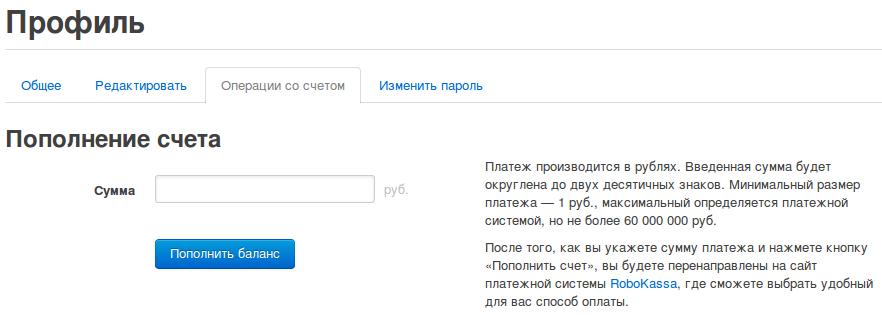
\includegraphics[width=\textwidth]{include/operations.png}
\caption{Форма пополнения счета рекламодателя.}
\label{fig:operations}
\end{figure}

Теперь на вашем счету есть средства для начала работы. Если вы предпочитаете другие способы перевода денежных средств, пожалуйста, свяжитесь с вашим менеджером.

\subsection{Загрузка рекламных материалов}

Для того, чтобы партнеры более продуктивно рекламировали ваши товары или услуги, можно загрузить рекламные материалы в созданную кампанию. Для этого необходимо перейти во вкладку <<Рекламные материалы>> на странице с описанием рекламной кампании.

Рекламные материалы можно загрузить с помощью формы, изображенной на рис.~\ref{fig:materials}. Принимаются изображения в форматах JPG (JPEG), GIF, PNG, SWF (Flash), SVG. Максимальный размер изображения~--- 1Мб.

\begin{figure}[!ht]
\centering
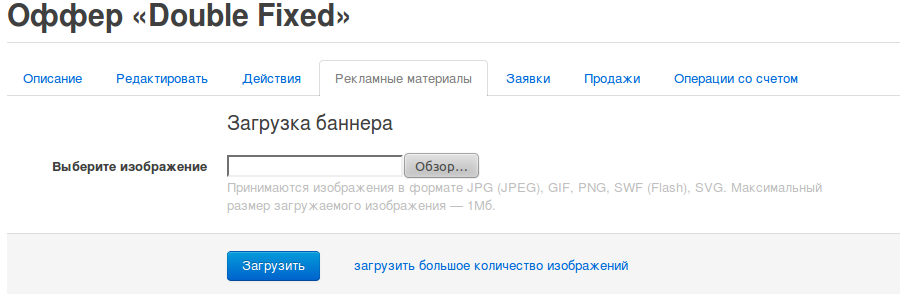
\includegraphics[width=\textwidth]{include/materials.png}
\caption{Форма загрузки рекламных материалов.}
\label{fig:materials}
\end{figure}

Для загрузки большого количества баннеров удобнее использовать форму мультизагрузки. Для этого перейдите по ссылке <<загрузить большое количество изображений>>.

\subsection{Запуск рекламной кампании}

После того, как вы заключили договор с \heymoose{}, сформировали список товаров в формате YML, реализовали сохранение токенов и XML-сервис, а также загрузили необходимые материалы, ваша рекламная кампания будет переведена в рабочее состояние. Это означает, что партнёры увидят описание кампании в каталоге офферов и смогут подать заявку на сотрудничество с рекламной кампанией.

\section{Сверка выполненных действий}

По прошествии некоторого времени после запуска рекламной кампании начнут отслеживаться заказы пользователей, перешедших от партнёров сети \heymoose{}. Вы можете увидеть их в списке продаж в личном кабинете рекламодателя. Для этого перейдите во вкладку <<Продажи>> страницы описания оффера (рис.~\ref{fig:sales}). Каждая строка таблицы означает покупку одного товара пользователем.

\begin{figure}[!ht]
\centering
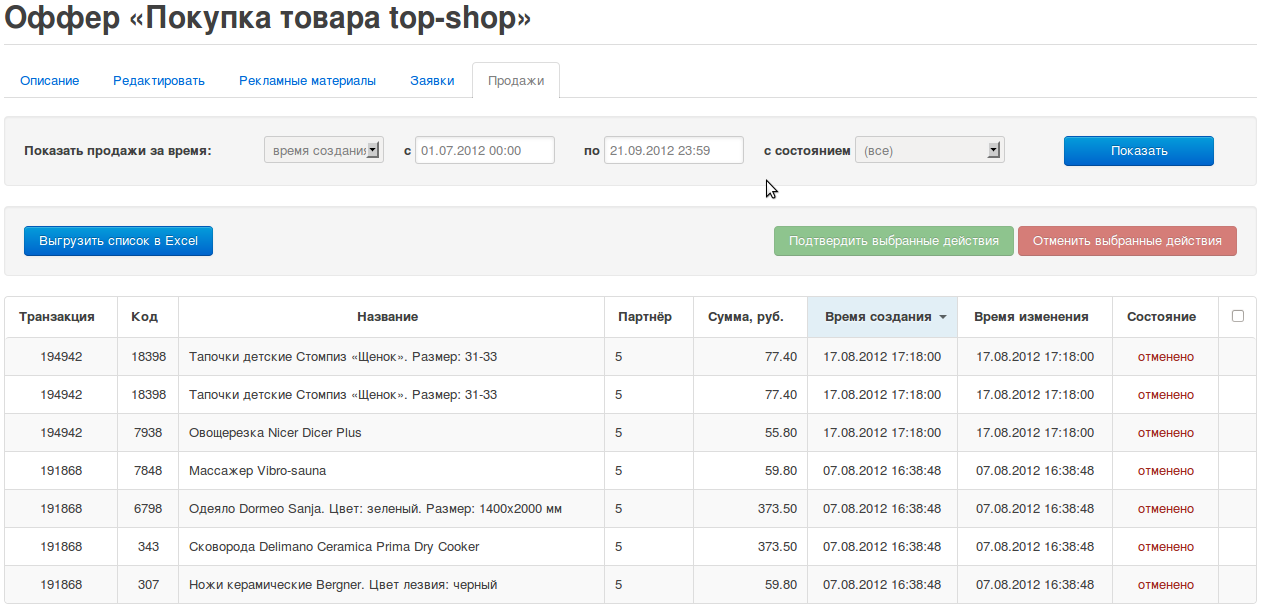
\includegraphics[width=\textwidth]{include/sales.png}
\caption{Список продаж по рекламной кампании.}
\label{fig:sales}
\end{figure}

В колонке <<Транзакция>> списка продаж находятся значения элемента \textbf{<transaction>}, переданные посредством XML-сервиса при создании заказа. В колонке <<Код>> находятся идентификаторы товаров (значения элементов \textbf{<id>} сервиса). По этим данным можно проводить сверку списка продаж в системе \heymoose{} со внутренней статистикой вашего сайта.

Для удобства сверки существует возможность выгрузки списка продаж за определенный период в формат XLS (электронную таблицу Microsoft Excel). Выберите интересующий вас период, фильтр по состоянию и нажмите кнопку <<Показать>>. После того, как отобразится список продаж, нажмите кнопку <<Выгрузить список в Excel>>. В полученном файле будут отображены все найденные продажи.

Процесс сверки подразумевает два основных действия: \textit{подтверждение} и \textit{отмену} товаров. Подтверждение товара означает, что этот товар был оплачен покупателем, и за него спишется вознаграждение партнёру. Для того, чтобы подтвердить товары, выберите их с помощью флажков справа и нажмите кнопку <<Подтвердить выбранные действия>>. Выбранные товары получат статус <<подтверждено>>.

Если при сверке оказалось, что некоторые товары отменены или некорректны, их можно отменить с помощью того же списка продаж. Для этого выберите необходимые товары с помощью флажков справа и нажмите кнопку <<Отменить выбранные действия>>. Выбранные товары получат статус <<отменено>>, а списанные за них средства вернутся на счет оффера.

Стоит подчеркнуть, что возможность отмены пропадает после того, как по заказу заканчивается холд. Подтвержденные заказа отменить также невозможно.

\section{Блокировка партнёров}

В списке продаж также можно наблюдать идентификаторы партнёров, от которых совершаются те или иные действия. Если вы заметили, что какой-то партнёр занимается накруткой трафика, использует нелегальные методы или действует подозрительно, вы можете запретить этому партнёру сотрудничать с вашей рекламной кампанией. Для этого перейдите во вкладку <<Заявки>> страницы описания оффера (рис.~\ref{fig:requests}).

\begin{figure}[!ht]
\centering
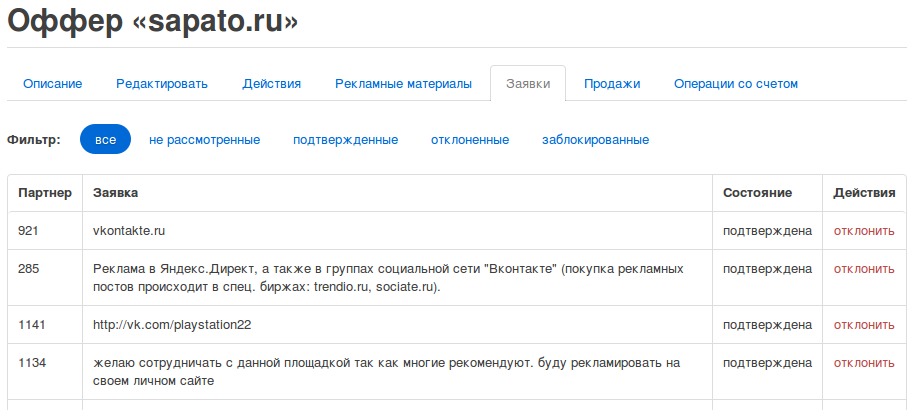
\includegraphics[width=\textwidth]{include/requests.png}
\caption{Список заявок на сотрудничество с рекламной кампанией.}
\label{fig:requests}
\end{figure}

Найдите заявку от партнёра с нужным идентификатором и нажмите кнопку <<отклонить>>. Более этот партнёр не сможет лить трафик на вашу рекламную кампанию.

Заявку можно в любой момент вернуть в прежнее состояние с помощью того же списка.

\section{Просмотр статистики}

Система \heymoose{} также предоставляет несколько срезов статистики для более удобного просмотра агрегированной информации по рекламным площадкам. Статистика обновляется в режиме реального времени.

Реализованы следующие срезы статистики:

\begin{itemize}
\item по офферам (рис.~\ref{fig:stats-offer});
\item по партнёрам (рис.~\ref{fig:stats-aff}).
\end{itemize}

\begin{figure}[!ht]
\centering
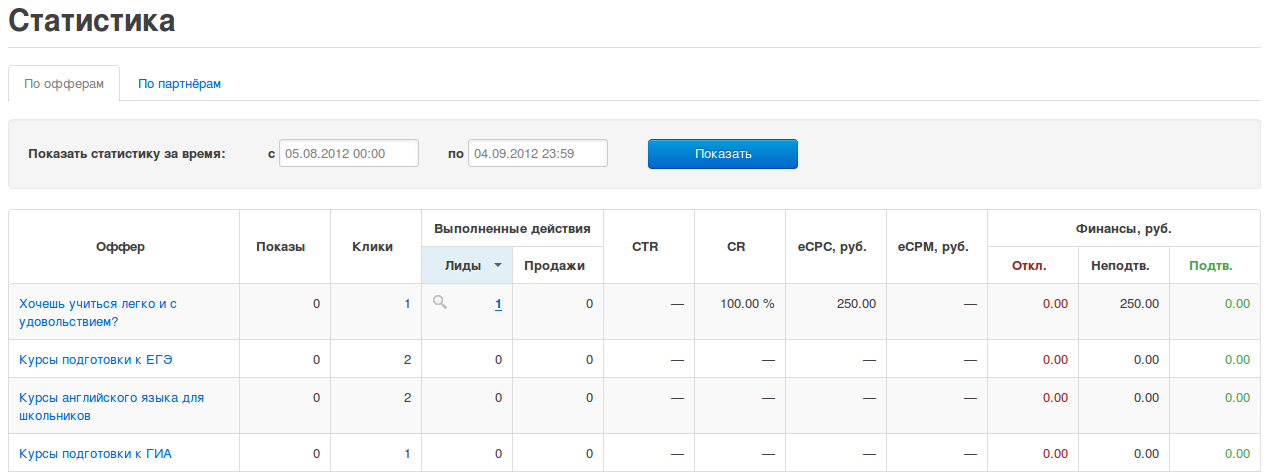
\includegraphics[width=\textwidth]{include/stats-offer.png}
\caption{Статистика по офферам.}
\label{fig:stats-offer}
\end{figure}

\begin{figure}[!ht]
\centering
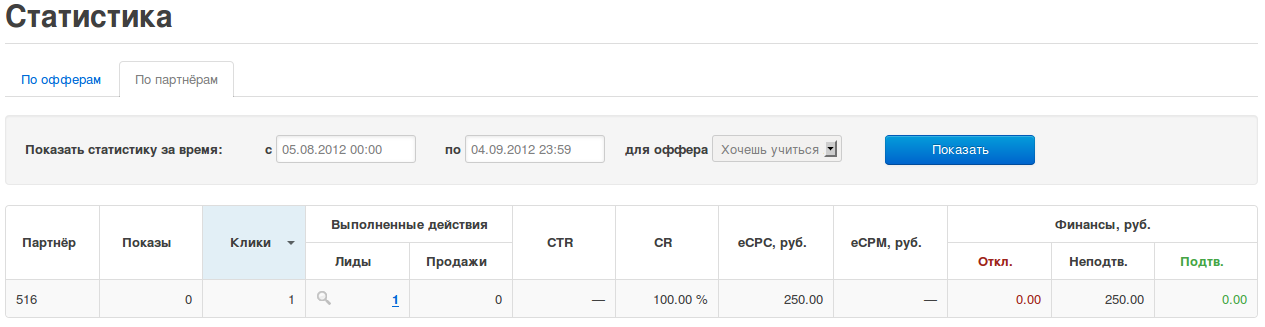
\includegraphics[width=\textwidth]{include/stats-aff.png}
\caption{Статистика по партнёрам.}
\label{fig:stats-aff}
\end{figure}

Помимо этого, кликнув на число лидов или продаж в каждой строке статистики, можно увидеть более развернутую информацию о том, какие именно товары были куплены (рис.~\ref{fig:stats-suboffer}).

\begin{figure}[!ht]
\centering
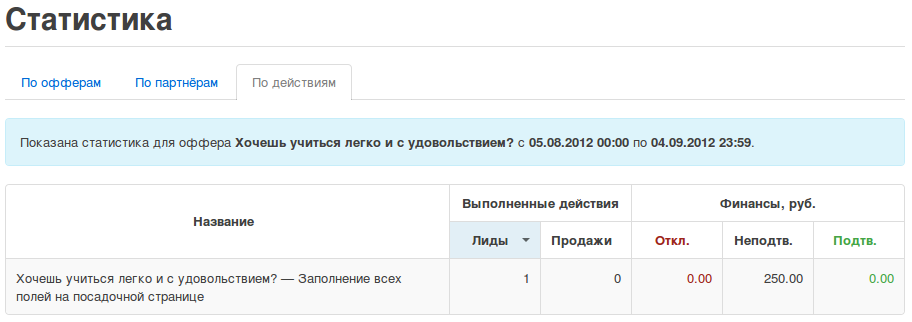
\includegraphics[width=\textwidth]{include/stats-suboffer.png}
\caption{Статистика по действиям.}
\label{fig:stats-suboffer}
\end{figure}

\end{document}
